% arara: pdflatex
% !arara: animate: {delay: 80}
% !arara: indent: {overwrite: yes, localSettings: yes}
\documentclass[mathserif, 14pt, xcolor=svgnames]{beamer}
\input{embed_video.tex}
%\documentclass[handout,mathserif]{beamer}
\usepackage{physics, amsmath,amsfonts,amsthm,amssymb, mathtools,steinmetz, gensymb, siunitx}	
\usepackage{caption}
%\usepackage{setspace}
\usepackage{pgf,tikz,pgfplots,wrapfig, graphicx}
\usepackage{rotating}
\usepackage{fancyhdr}
\usepackage{float}
\usepackage{listings}
\usepackage{array}
\usepackage{booktabs,multirow}
\usepackage{bm}
\usepackage{url}  % to handle urls
\usepackage[comma,authoryear]{natbib}  % for authordate ref style --  allows \citet (textual), and \citep (parenthesized)
\usepackage{hyperref}
\usepackage{pifont}


\newcommand{\tfont[1]}{ #1}

\renewcommand {\cite} {\citep}  % default for cite is citet in natbib - so change it
\renewcommand\bibname{References}    % if not using newrucsthesis sty file
\bibpunct[, ]{(}{)}{;}{a}{,}{,}

\renewcommand {\thempfootnote} {\arabic{mpfootnote}}  % default for cite is citet in natbib - so change it

\usetikzlibrary{positioning}
\usetikzlibrary{fit}
\usetikzlibrary{backgrounds}
\usetikzlibrary{calc}
\usetikzlibrary{shapes}
\usetikzlibrary{mindmap}
\usetikzlibrary{decorations.text}
\pgfplotsset{compat=1.7}
\usepackage{tikz}

\definecolor{coolblack}{rgb}{0.0, 0.18, 0.39}
\definecolor{OxfordBlue}{rgb}{0.0, 0.082, 0.21}
\definecolor{Tangerine}{rgb}{0.95, 0.52, 0.0}
\definecolor{Tangelo}{rgb}{0.98, 0.35, 0.0}

\newcommand\blfootnote[1]{
  \begingroup
  \renewcommand\thefootnote{}\footnote{#1}
  \addtocounter{footnote}{-1}
  \endgroup
}
%\renewcommand*{\bibfont}{\tiny}

\newcommand{\topline}{%
  \tikz[remember picture,overlay] {%
    \draw[Tangerine,ultra thick] ([yshift=-1.6em]current page.north west)-- ([yshift=-1.6em,xshift=\paperwidth]current page.north west);}}

\addtobeamertemplate{frametitle}{}{\topline%
}

% tikzmark command, for shading over items
\newcommand{\tikzmark}[1]{\tikz[overlay,remember picture] \node (#1) {};}

\setbeamercolor{frametitle}{fg=white}

% title color
\setbeamercolor{title}{fg=white}
\setbeamercolor{footnote mark}{fg=.}
\setbeamercolor{normal text}{fg=white}

% standard enumeration
\setbeamertemplate{enumerate items}{(\arabic{enumi})}

% color of slides
\setbeamercolor{background canvas}{bg=OxfordBlue}

% color of references
\setbeamercolor{bibliography item}{fg=white}
\setbeamercolor{bibliography entry title}{fg=white}
\setbeamercolor{bibliography entry author}{fg=white}
\setbeamercolor{bibliography entry date}{fg=white}
\setbeamercolor{bibliography entry note}{fg=white}
\setbeamercolor{bibliography entry url}{fg=white}
\setbeamercolor{bibliography entry organiation}{fg=white}
\setbeamercolor{bibliography entry location}{fg=white}
%
%\setbeamerfont{bibliography item}{size=\tiny}
%\setbeamerfont{bibliography entry title}{size=\tiny}
%\setbeamerfont{bibliography entry author}{size=\tiny}
%\setbeamerfont{bibliography entry date}{size=\tiny}
%\setbeamerfont{bibliography entry note}{size=\tiny}
%\setbeamerfont{bibliography entry url}{size=\tiny}
%\setbeamerfont{bibliography entry organization}{size=\tiny}
%\setbeamerfont{bibliography entry location}{size=\tiny}
%
% default itemize
\setbeamertemplate{itemize items}[circle]

% no navigation symbols
\setbeamertemplate{navigation symbols}{}

\setbeamercolor{itemize item}{fg=Tangelo}
\setbeamertemplate{itemize item}{\maltese}
\setbeamercolor{itemize subitem}{fg=Tangelo}
\setbeamertemplate{itemize subitem}{\begin{rotate}{90}$\diamondsuit$\end{rotate}}

\usepackage[T1]{fontenc}
%\usepackage{fontspec}
%\setmainfont{TeX Gyre Pagella}%% The Palatino from the TeX Gyre Project

% transparency
\setbeamercovered{invisible}

% for resuming lists across frames
\newcounter{savedenum}
\newcommand*{\saveenum}{\setcounter{savedenum}{\theenumi}}
\newcommand*{\resume}{\setcounter{enumi}{\thesavedenum}}

% title
\title{Tracking and Detection of Multiple Human Faces }
\subtitle{}

\author[Gouws]{J L Gouws\inst{1}\\[1ex]  \and {\small Supervisor: Mr. J Connan\inst{1}}}
\date{\today}
\institute[RU]{\inst{1} Rhodes University}
\tikzset{
   invisible/.style={opacity=0},
   visible on/.style={alt=#1{}{invisible}},
   alt/.code args={<#1>#2#3}{%
      \alt<#1>{\pgfkeysalso{#2}}{\pgfkeysalso{#3}} % \pgfkeysalso doesn't change the path
   },
}

%\includeonlyframes{daytoday}

\begin{document}

\begin{frame}
   \maketitle
\end{frame}

\usetikzlibrary{shapes.geometric, arrows}

\tikzstyle{startstop} = [draw, line width = 0.2em, fill = white, rectangle, rounded corners, minimum width=3cm, minimum height=1cm,text centered, text = black]
\tikzstyle{io} = [draw, line width = 0.2em, text = black, trapezium, trapezium left angle=70, trapezium right angle=110, minimum width=3cm, minimum height=1cm, text centered, draw=black]
\tikzstyle{process} = [draw, line width = 0.2em, text = black, rectangle, minimum width=3cm, minimum height=1cm, text centered, draw=black]
\tikzstyle{decision} = [diamond, aspect = 2.5,minimum width=2cm, minimum height=0.5cm, text centered, draw=black]
\tikzstyle{arrow} = [line width = 0.2em,->,>=stealth]
\tikzstyle{line} = [thick]

\bgroup
\begin{frame}{Presentation Overview}
  \centering
  \begin{tikzpicture}[node distance=3em]
    \pause
    \node (ps) [startstop, draw = Chartreuse, fill = Chartreuse!10] {Problem Statement};
    \pause
    \node (litRev) [io, draw = Salmon, fill = Salmon!20, below of=ps] {Literature Review};
    \draw[arrow] (ps) -- (litRev);
    \pause
    \node (progress) [process, draw = Goldenrod, fill = Goldenrod!20, below of=litRev] {Progress};
    \draw[arrow] (litRev) -- (progress);
    \pause
    \node (future) [io, draw = DarkSeaGreen, fill = DarkSeaGreen!20, below of=progress] {Going Foward};
    \draw[arrow] (progress) -- (future);
    \pause
    \node (qs) [startstop, draw = Red, fill = Red!30, below of=future] {Questions};
    \draw[arrow] (future) -- (qs);

  \end{tikzpicture}
\end{frame}
\egroup

\bgroup
\begin{frame}{Problem Statement}
  \begin{minipage}[t]{\textwidth}
  { \Large
    The design and implementation of a long-term tracking system--given minimal input data,
    the system can identify multiple target faces per video stream frame--can use the TLD\footnotemark[1] framework.
  }
  \end{minipage}
  \footnotetext[1]<3->{\citep{KalalPHD}}
\end{frame}
\egroup

\bgroup
\begin{frame}{Objectives}
  \begin{itemize}
     \setlength\itemsep{1.2em}
    \item \hspace{0pt}
      \pause Improve TLD's ST tracking performance
    \item \hspace{0pt}
      \pause Adapt TLD to track faces specifically
    \item \hspace{0pt}
      \pause
        Multiple faces with single tracker
    \item \hspace{0pt}
      \pause
        Evaluate single face tracking performance
    \item \hspace{0pt}
      \pause
        Re-evaluate for multiple targets
  \end{itemize}
\end{frame}
\egroup

\bgroup

\begin{frame}{Proposed system}
  \begin{center}
  \resizebox{\textwidth}{!}{
       \begin{tikzpicture}[approach/.style={draw,very thick, fill=white, text width=5em,
             text centered, minimum height=2em,rounded corners=3ex},
             idea/.style={draw=yellow, circle,text width=5em,
                text centered, minimum height=2.5em},
              filter/.style={draw=yellow, ellipse, text width=8em,
                text centered, minimum height=1em},
              sect/.style={draw=yellow, ellipse, text width=7em,
                text centered, minimum height=1em},
              layer/.style={draw=yellow, circle,text width=1em,
                text centered, minimum height=1em},
             connections/.style={->,draw=yellow,shorten <=2pt,shorten >=2pt},
             reverseConnections/.style={<-,draw=yellow,shorten <=2pt,shorten >=2pt},
          ]
          
          \node[draw] at (0,3) (all) [filter]  {Input Image};
          \node[draw] at (0,0) (l1) [filter]  {Face-Detector};
          \node[draw] at (3,-4) (l2) [sect]  {Random\\Forest};
          \node[draw] at (2.8,-7) (l3) [sect, text width=4.5em]  {NN\\Classifier};
          \node[draw] at (9,-1.5) (l4) [filter]  {KCF\\tracker};
          \node[draw] at (-3,-4) (l5) [sect]  {Random\\Forest};
          \node[draw] at (-2.7,-7) (l6) [sect, text width=4.5em]  {NN\\Classifier};
          \node[draw] at (-9,-1.5) (l7) [filter]  {KCF\\tracker};
          \node[draw] at (2,-9) (l8) [sect, text width=4em]  {Face};
          \node[draw] at (-2,-9) (l9) [sect, text width=4em]  {Face};
          \draw[connections] (all.south) -- (l1.north) ;
          \draw[connections] (all.south) -- (l4.north);
          \draw[connections] (all.south) -- (l7.north);
          \draw[reverseConnections, postaction={decorate, decoration={raise=1.5ex, text along path, text align={left indent={0.1\dimexpr\pgfdecoratedpathlength\relax}}, text color = orange, text={Bootsrap}}}] (l2.east)  -- (l4.south);
          \draw[reverseConnections, postaction={decorate, decoration={raise=1.5ex, text along path, text align={left indent={0.2\dimexpr\pgfdecoratedpathlength\relax}}, text color = orange, text={Bootsrap}}}] (l3.east) -- (l4.south);
          \draw[connections] (l1.south) -- (l2.north) ;
          \draw[connections] (l2.south) -- (l3.north) ;
          \draw[connections, postaction={decorate, decoration={raise=1.5ex, text along path, text align={left indent={0.4\dimexpr\pgfdecoratedpathlength\relax}}, text color = orange, text={Bootsrap}}}] (l7.south) -- (l5.west) ;
          \draw[connections, postaction={decorate, decoration={raise=1.5ex, text along path, text align={left indent={0.5\dimexpr\pgfdecoratedpathlength\relax}}, text color = orange, text={Bootsrap}}}] (l7.south) -- (l6.west) ;
          \draw[connections] (l1.south) -- (l5.north) ;
          \draw[connections] (l5.south) -- (l6.north) ;
          \draw[connections] (l3.south) -- (l8.north) ;
          \draw[connections] (l6.south) -- (l9.north) ;
          
          
       \end{tikzpicture}
  }
  \end{center}
\end{frame}
\egroup

\bgroup
\begin{frame}{KCF Tracker \cite{Enriques2014}}
   \begin{itemize}
     \setlength\itemsep{1.2em}
     \item \hspace{0pt}
       \pause Ridge Regression Confidence
     \item \hspace{0pt}
       \pause 
        \begin{equation*}
          f(\pmb{z}) = \pmb{w}^T\pmb{z} = \sum_{i = 1}^n \alpha_i \kappa(\pmb{z}, \pmb{x}_i)   
        \end{equation*}
     \item \hspace{0pt}
       \pause Fail if $f(\pmb{z}) < f_{\text{min}}$
    \end{itemize}
\end{frame}
\egroup


\bgroup

\begin{frame}{Face Detector}
   \begin{itemize}
     \setlength\itemsep{1.2em}
     \item \hspace{0pt}
       \pause IoU relates Face Detector and Sliding Window
     \item \hspace{0pt}
       \pause SSD \cite{liu2016}
       \begin{itemize}
           72.1 \% mAP on VOC2007
       \end{itemize}
     \item \hspace{0pt}
       \pause Haar Cascade \cite{viola2001}
    \end{itemize}
\end{frame}

\egroup

\bgroup
\begin{frame}{Experiment 1}

    \begin{itemize}
      \setlength\itemsep{1.3em}
       \item \hspace{0pt}
         \pause Investigate KCF effect's on ST tracking performance
       \item \hspace{0pt}
         \pause Use OTB subset \cite{OTBDataset}
       \item \hspace{0pt}
         \pause Determine $f_\text{min}$'s effect on ST tracking
       \item \hspace{0pt}
         \pause Compare KCF and MFT as ST tracker
    \end{itemize}
\end{frame}
\egroup

\bgroup
\begin{frame}{Experiment 1}
  \begin{table}
  \resizebox{\textwidth}{!}{
            \begin{tabular}[]{
                                @{}l 
                                @{\hspace*{2em}} c 
                                @{\hspace*{2em}} c 
                                @{\hspace*{2em}} c 
                                @{\hspace*{2em}} c 
                                @{\hspace*{2em}} c}
                \toprule
                Method      & $\phi_\text{min}$ & precision & recall    & F-score & Average Overlap\\
                \midrule
                Median Flow & NA                & 0.7186         & 0.8562 & 0.7406 & 0.5206\\
                \hline
                KCF         & 0.3               & 0.8790       & 0.6631 & 0.7186 & 0.4735\\
                \hline
                KCF         & 0.25              & 0.8790       & 0.7646 & 0.7810 & 0.5227\\
                \hline
                KCF         & 0.20              & 0.0.7994       & 0.9221 & 0.8425 & 0.6289\\
                \hline
                KCF         & 0.17              & 0.8532       & 0.9565 & 0.8953 & 0.6600\\
                \hline
                KCF         & 0.15              & 0.8997       & 0.9498 & 0.9225 & 0.6714\\
                \hline
                KCF         & 0.13              & 0.8880      & 0.9679 & 0.9225 & 0.6749\\
                \hline
                KCF         & 0.11              & 0.8911      & 0.9986 & 0.9323 & 0.6822\\
                \hline
                KCF         & 0.09              & 0.8909      & 1.0 & 0.9323 & 0.6822\\
                \bottomrule
            \end{tabular}
}
    \caption{The ST Tracker's Effect on Average Performance Metrics }
    \label{tab:exp1}
  \end{table}
\end{frame}
\egroup

\bgroup
\begin{frame}{Experiment 1}
  \begin{center}
    \includegraphics[scale = 0.5]{sttracker.pdf}
  \end{center}
\end{frame}
\egroup

\bgroup
\begin{frame}{Experiment 2}

    \begin{itemize}
       \setlength\itemsep{1.2em}
       \item \hspace{0pt}
         \pause Investigate face detector's effect on ST tracking performance
       \item \hspace{0pt}
         \pause Use Same OTB subset
       \item \hspace{0pt}
         \pause Compare Haar Cascade and SSD
       \item \hspace{0pt}
         \pause Expect similar results to Experiment 1
    \end{itemize}
\end{frame}
\egroup

\bgroup
\begin{frame}{Experiment 2}
  \begin{table}
  \resizebox{\textwidth}{!}{
            \begin{tabular}[]{
                                @{}l 
                                @{\hspace*{2em}} c 
                                @{\hspace*{2em}} c 
                                @{\hspace*{2em}} c 
                                @{\hspace*{2em}} c 
                                @{\hspace*{2em}} c}
                \toprule
                Method      & precision & recall    & F-score & Average Overlap\\
                \midrule
                Variance    & 0.8997    & 0.9498 & 0.9225 & 0.6714\\
                \hline
                SSD         & 0.9406    & 0.9106 & 0.9541 & 0.6853\\
                \hline
                Haar        & 0.9228    & 0.9778 & 0.9481 & 0.6806\\
                \bottomrule
            \end{tabular}
}
    \caption{Face Detector's Effect on ST Tracking Performance}
%}
  \end{table}
\end{frame}
\egroup

\bgroup
\begin{frame}{Experiment 3}
    \begin{itemize}
       \setlength\itemsep{1.2em}
       \item \hspace{0pt}
         \pause Investigate tracker's LT tracking performance
       \item \hspace{0pt}
         \pause VOT video
       \item \hspace{0pt}
         \pause Compare Haar Cascade and SSD
    \end{itemize}
\end{frame}
\egroup


\bgroup
\begin{frame}{Experiment 3}
  \begin{table}
  \resizebox{\textwidth}{!}{
            \begin{tabular}[]{
                                @{}l 
                                @{\hspace*{2em}} c 
                                @{\hspace*{2em}} c 
                                @{\hspace*{2em}} c 
                                @{\hspace*{2em}} c 
                                @{\hspace*{2em}} c}
                \toprule
                Method      & precision & recall    & F-score\\
                \midrule
                Variance    & 0.9175    & 0.0286 & 0.0555\\
                \hline
                SSD         & 0.7743    & 0.7029 & 0.7369 \\
                \hline
                Haar        & 0.6184    & 0.5858 & 0.6016\\
                \bottomrule
            \end{tabular}
}
        \caption{Performance Metrics for LT Sequence}
  \end{table}
\end{frame}
\egroup

\bgroup
\begin{frame}{Experiment 4}
    \begin{itemize}
      \setlength\itemsep{1.2em}
       \item \hspace{0pt}
         \pause Multiple Face tracking performance
       \item \hspace{0pt}
         \pause Two Hand Labelled Videos
       \item \hspace{0pt}
         \pause Compare Haar Cascade and SSD
    \end{itemize}
\end{frame}
\egroup

\bgroup
\begin{frame}{Experiment 4}
  \begin{center}
    \includegraphics[scale = 0.25]{precRecallCurvesDnn.pdf} \\
    \includegraphics[scale = 0.25]{precRecallCurvesVan.pdf}
  \end{center}
\end{frame}
\egroup

\bgroup
\begin{frame}{Experiment 4}
  \begin{table}
  \resizebox{\textwidth}{!}{
            \begin{tabular}[]{
                                @{}l 
                                @{\hspace*{2em}} c 
                                @{\hspace*{2em}} c 
                                @{\hspace*{2em}} c 
                                @{\hspace*{2em}} c 
                                @{\hspace*{2em}} c}
                \toprule
                Method      & Video & mAP/ \% \\
                \midrule
                Variance    & Berrwam    & 23.03\\
                \hline
                SSD         & Berrywam   & 74.87 \\
                \hline
                Haar        & Berrywam   & 67.45\\
                \hline
                Variance    & Pentatonix & 33.58\\
                \hline
                SSD         & Pentatonix & 71.83 \\
                \hline
                Haar        & Pentatonix & 56.38\\
                \bottomrule
            \end{tabular}
}
        \caption{mean Average Precision for Various Tracker Implementations}
  \end{table}
\end{frame}
\egroup

\bgroup
\begin{frame}{Experiment 4}
  \begin{center}
      \embedvideo*{\includegraphics[width=\textwidth]{tldOUT.jpg}}{tldOUT.mp4}
  \end{center}
\end{frame}
\egroup

\begin{frame}{References}
    \bibliographystyle{ruauthordate}
    \fontsize{6pt}{6pt}\selectfont
%    { \tiny
    \bibliography{references.bib}   	% load in the citation info from ref.bib
%    }
\end{frame}

\end{document}


%\iffalse
 %  \begin{columns}
 %     \begin{column}[t]{.65\textwidth}
 %        What tools do faculty use?
 %
 %        \begin{tikzpicture}[every node/.append style={align=center}]
 %           \begin{pgfonlayer}{background}
 %              \node[circle,fill=red!30,draw=black,thick,minimum size=5cm](0,0){Microsoft Word\\ 86\%};
 %           \end{pgfonlayer}{background}
 %           \pause
 %              \visible<2->{\filldraw[gray,opacity=0.5] (2.5,0) arc (0:-190:2.5cm) -- (0,0)node[black,opacity=1,anchor=north east,scale=1,inner sep=.5cm] {MathType \\ 60\%};}
 %           \pause
 %              \visible<3->{\node[circle,fill=blue!40,draw=black,scale=1.15] at (2.3,-1){\LaTeX\\16\%};}
 %           \pause
 %              \visible<4->{\node[circle,fill=orange!40,draw=black,scale=0.65] at (2.3,1){Open Office\\12\%};}
 %        \end{tikzpicture}
 %     \end{column}%
 %\fi

\begin{frame}{Rule of four}

   \centering
   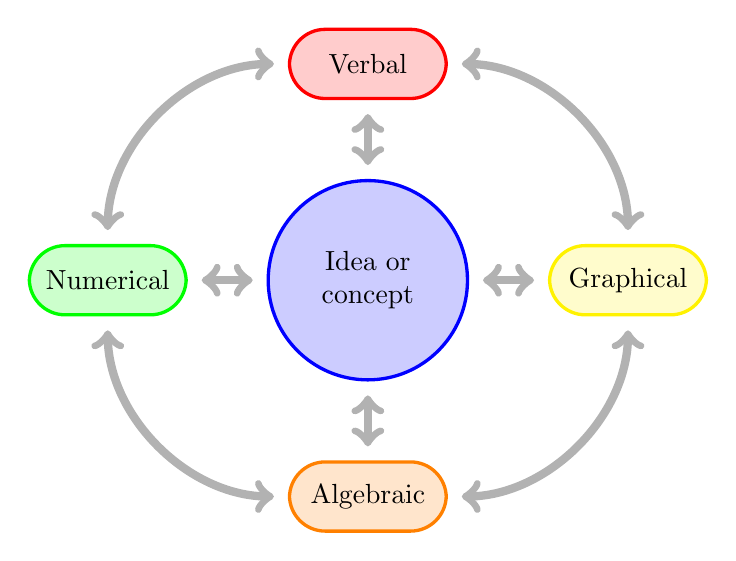
\begin{tikzpicture}[approach/.style={draw,very thick, fill=blue!20, text width=5em,
            text centered, minimum height=2.5em,rounded corners=3ex},
         idea/.style={draw, very thick,fill=blue!40, circle,text width=6em,
            text centered, minimum height=2.5em},
         connections/.style={<->,draw=black!30,line width=3pt,shorten <=5pt,shorten >=5pt},
      ]

      % Draw diagram elements
      \node (idea) [idea,draw=blue,fill=blue!20]  {Idea or concept};
      \pause
         \node (verbal) [approach,draw=red,fill=red!20,above=of idea]  {Verbal};
         \node (tabular) [approach,draw=green,fill=green!20,left=of idea]  {Numerical};
         \node (graphical)[approach,draw=yellow,fill=yellow!20,right=of idea] {Graphical};
         \node (formular)[approach,draw=orange,fill=orange!20,below=of idea] {Algebraic};

         % Draw arrows between elements
         \draw[connections] (idea) -- (formular) ;
         \draw[connections] (idea) -- (verbal);
         \draw[connections] (idea) -- (graphical);
         \draw[connections] (idea) -- (tabular);
         \draw[connections] (verbal.west) to[out=180,in=90](tabular.north) ;
         \draw[connections] (verbal.east) to[out=0,in=90](graphical.north) ;
         \draw[connections] (tabular.south) to[out=-90,in=180](formular.west) ;
         \draw[connections] (graphical.south)to[out=-90,in=0](formular.east);
   \end{tikzpicture}

\end{frame}

\begin{frame}[label=workflow]{Workflow}

   \makebox[\textwidth][c]{%
      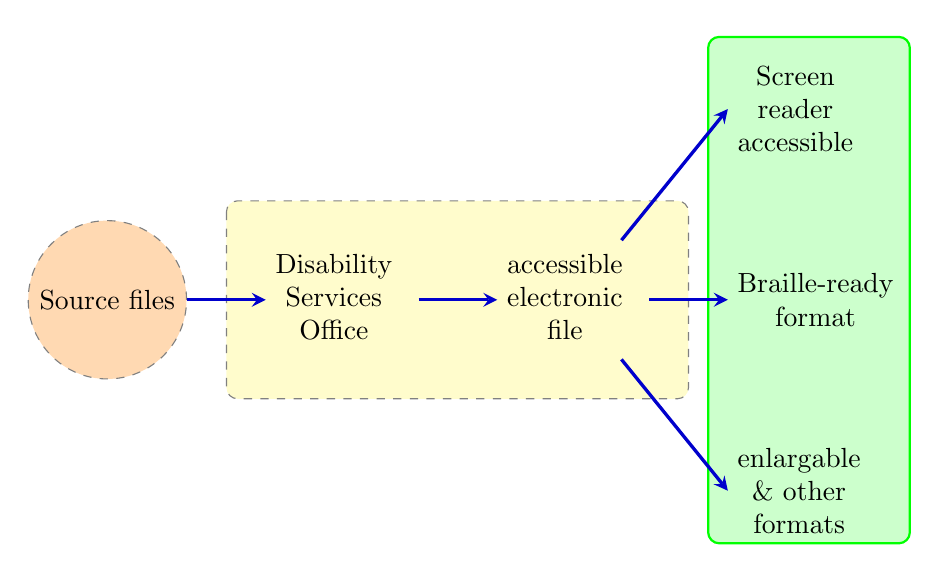
\begin{tikzpicture}[
            outpt/.style={->,blue!80!black,very thick},
            >=stealth,
         every node/.append style={align=center}]
         \node (kaela) at (0,0) {\begin{tabular}{@{}c}Disability\\ Services \\ Office \end{tabular}};
         \pause
            \node (accessfile) [right=of kaela] {\begin{tabular}{@{}c}accessible\\ electronic \\ file \end{tabular}};
            \draw[outpt](kaela)--(accessfile);
            % Draw background
            \begin{pgfonlayer}{background}
               % Left-top corner of the background rectangle
               \path (kaela.west |- kaela.north)+(-0.5,0.5) node (a) {};
               % Right-bottom corner of the background rectanle
               \path (accessfile.east |- accessfile.south)+(+0.5,-0.5) node (c) {};
               % Draw the background
               \path[fill=yellow!20,rounded corners, draw=black!50, dashed]
               (a) rectangle (c);
            \end{pgfonlayer}
         \pause
            \node (screen)[above right=of accessfile]{Screen\\ reader\\ accessible};
            \node (braille)[right =of accessfile]{Braille-ready\\ format};
            \node (enlarge)[below right=of accessfile]{enlargable\\ \& other \\ formats};
            \draw[outpt](accessfile)--(screen.west);
            \draw[outpt](accessfile)--(braille);
            \draw[outpt](accessfile)--(enlarge.west);
            \begin{pgfonlayer}{background}
               % Left-top corner of the background rectangle
               \path (screen.west |- screen.north)+(-0.25,0.25) node (a) {};
               % Right-bottom corner of the background rectanle
               \path (enlarge.east |- enlarge.south)+(0.5,0) node (c) {};
               % Draw the background
               \path[fill=green!20,rounded corners, draw=green,thick]
               (a) rectangle (c);
            \end{pgfonlayer}
         \pause
            \node (source) [left=of kaela,draw=black!50,dashed,circle,fill=orange!30]{Source files};
            \draw[outpt](source)--(kaela);
      \end{tikzpicture}
   }
\end{frame}

\begin{frame}{Stand alone concept}

   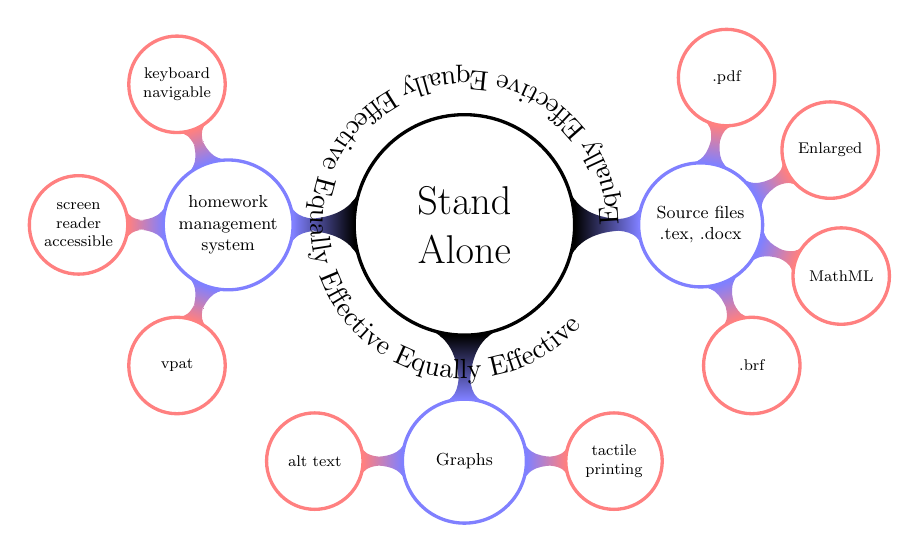
\begin{tikzpicture}[mindmap,
         concept/.append style={fill={none}},
         root concept/.style={concept color=blue},
         level 1 concept/.append style=
         {every child/.style={concept color=blue!50},level distance = 30mm},
         level 2 concept/.append style=
         {every child/.style={concept color=red!50},level distance = 19mm},
         every node/.append style={align=center,scale=0.7},
      ]
      \node [concept,font=\huge] {Stand\\ Alone}
      child[grow=0, visible on=<2->] {node[concept] {Source files .tex, .docx}
         child[grow=80, visible on=<2->]{node[concept] {.pdf}}
         child[grow=30, visible on=<2->]{node[concept] {Enlarged}}
         child[grow=-20, visible on=<2->]{node[concept] {MathML}}
         child[grow=-70, visible on=<2->]{node[concept] {.brf}}
      }
      child[grow=-90,visible on=<3->] {node[concept] {Graphs}
         child[grow=0,visible on=<3->]{node[concept] {tactile printing}}
         child[grow=180,visible on=<3->]{node[concept] {alt text}}
      }
      child[grow=180,visible on=<4->] {node[concept] {homework management system}
         child[grow=110,visible on=<4-> ] {node[concept] {keyboard navigable}}
         child[grow=180,visible on=<4->] {node[concept] {screen reader accessible}}
         child[grow=250,visible on=<4->] {node[concept] {vpat}}
      };
      \node at (0,0) [inner sep=9mm,decorate,circle,decoration=
      {text along path,text={Equally Effective Equally Effective Equally Effective  Equally Effective }}] {};
      %\draw decorate[decoration={text along path,text={Equally Effective}}]
      %{(-3,0) arc (135:45:.5cm)};

   \end{tikzpicture}
\end{frame}

\begin{frame}[c]{What stands alone?}
   % Which content creation tools stand alone?
   \pause
   \begin{columns}
      \begin{column}[c]{.33\textwidth}
         \tikz \node[fill=green!20,draw=green, rounded corners,very thick,inner sep=0mm]{%
            \vbox{%
               \begin{itemize}
                  \item MS Word with MathType
                  \item \LaTeX
                  \item LibreOffice
                  \item Scientific Notebook
                  \item Graphs
                  \item Prepared lecture notes
                  \item Desire2Learn
                  \item WeBWorK
                  \item Videos
               \end{itemize}
            }%
         };
      \end{column}%
      \pause
         \begin{column}[c]{.33\textwidth}
            \tikz \node[fill=orange!20,draw=orange, rounded corners,very thick,inner sep=0mm]{%
               \vbox{%
                  \begin{itemize}
                     \item[] MyMathLab
                  \end{itemize}
               }
            };
            \vfill
         \end{column}%
      \pause
         \begin{column}[c]{.33\textwidth}
            \tikz \node[fill=red!20,
               draw=red,
               rounded corners,
               very thick,
               inner sep=0mm,
               %decorate,decoration={zigzag,segment length=10mm,amplitude=2.0mm},
            ]{%
               \vbox{%
                  \begin{itemize}
                     \item MS Word OMML
                     \item PowerPoint
                     \item TestGen
                     \item GeoGebra applets
                     \item Flash-based applets
                     \item Other media
                  \end{itemize}
               }
            };
         \end{column}
   \end{columns}

\end{frame}


\begin{frame}[fragile]{Collaboration is key}
   \makebox[\textwidth][c]{%
      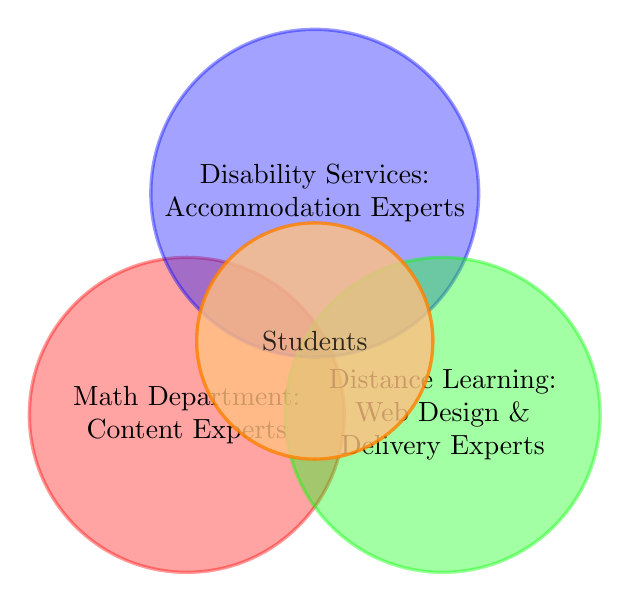
\begin{tikzpicture}[venn circle/.style={draw=#1,
               circle,
               very thick,
               minimum width=4cm,
               text=black,
               fill=#1!90,
               opacity=0.4,
               text opacity=1},
         every node/.append style={align=center}]
         \node [venn circle = red] (A) at (0,0) {Math Department:\\ Content Experts};
         \visible<2->{\node [venn circle = blue] (B) at (60:3.25cm) {Disability Services:\\ Accommodation Experts};}
         \visible<3->{\node [venn circle = green] (C) at (0:3.25cm) {Distance Learning:\\ Web Design \&\\Delivery Experts};}
         \visible<4->{\node[circle,fill=orange!50,draw=orange,very thick,opacity=0.8,minimum width=3cm] at (barycentric cs:A=1/3,B=1/3,C=1/3 ){Students};}
      \end{tikzpicture}
   }
\end{frame}
